% Figure: SNR + Invariant Residual adaptive payload architecture (EXP-034)
\begin{figure}[!htbp]
\centering
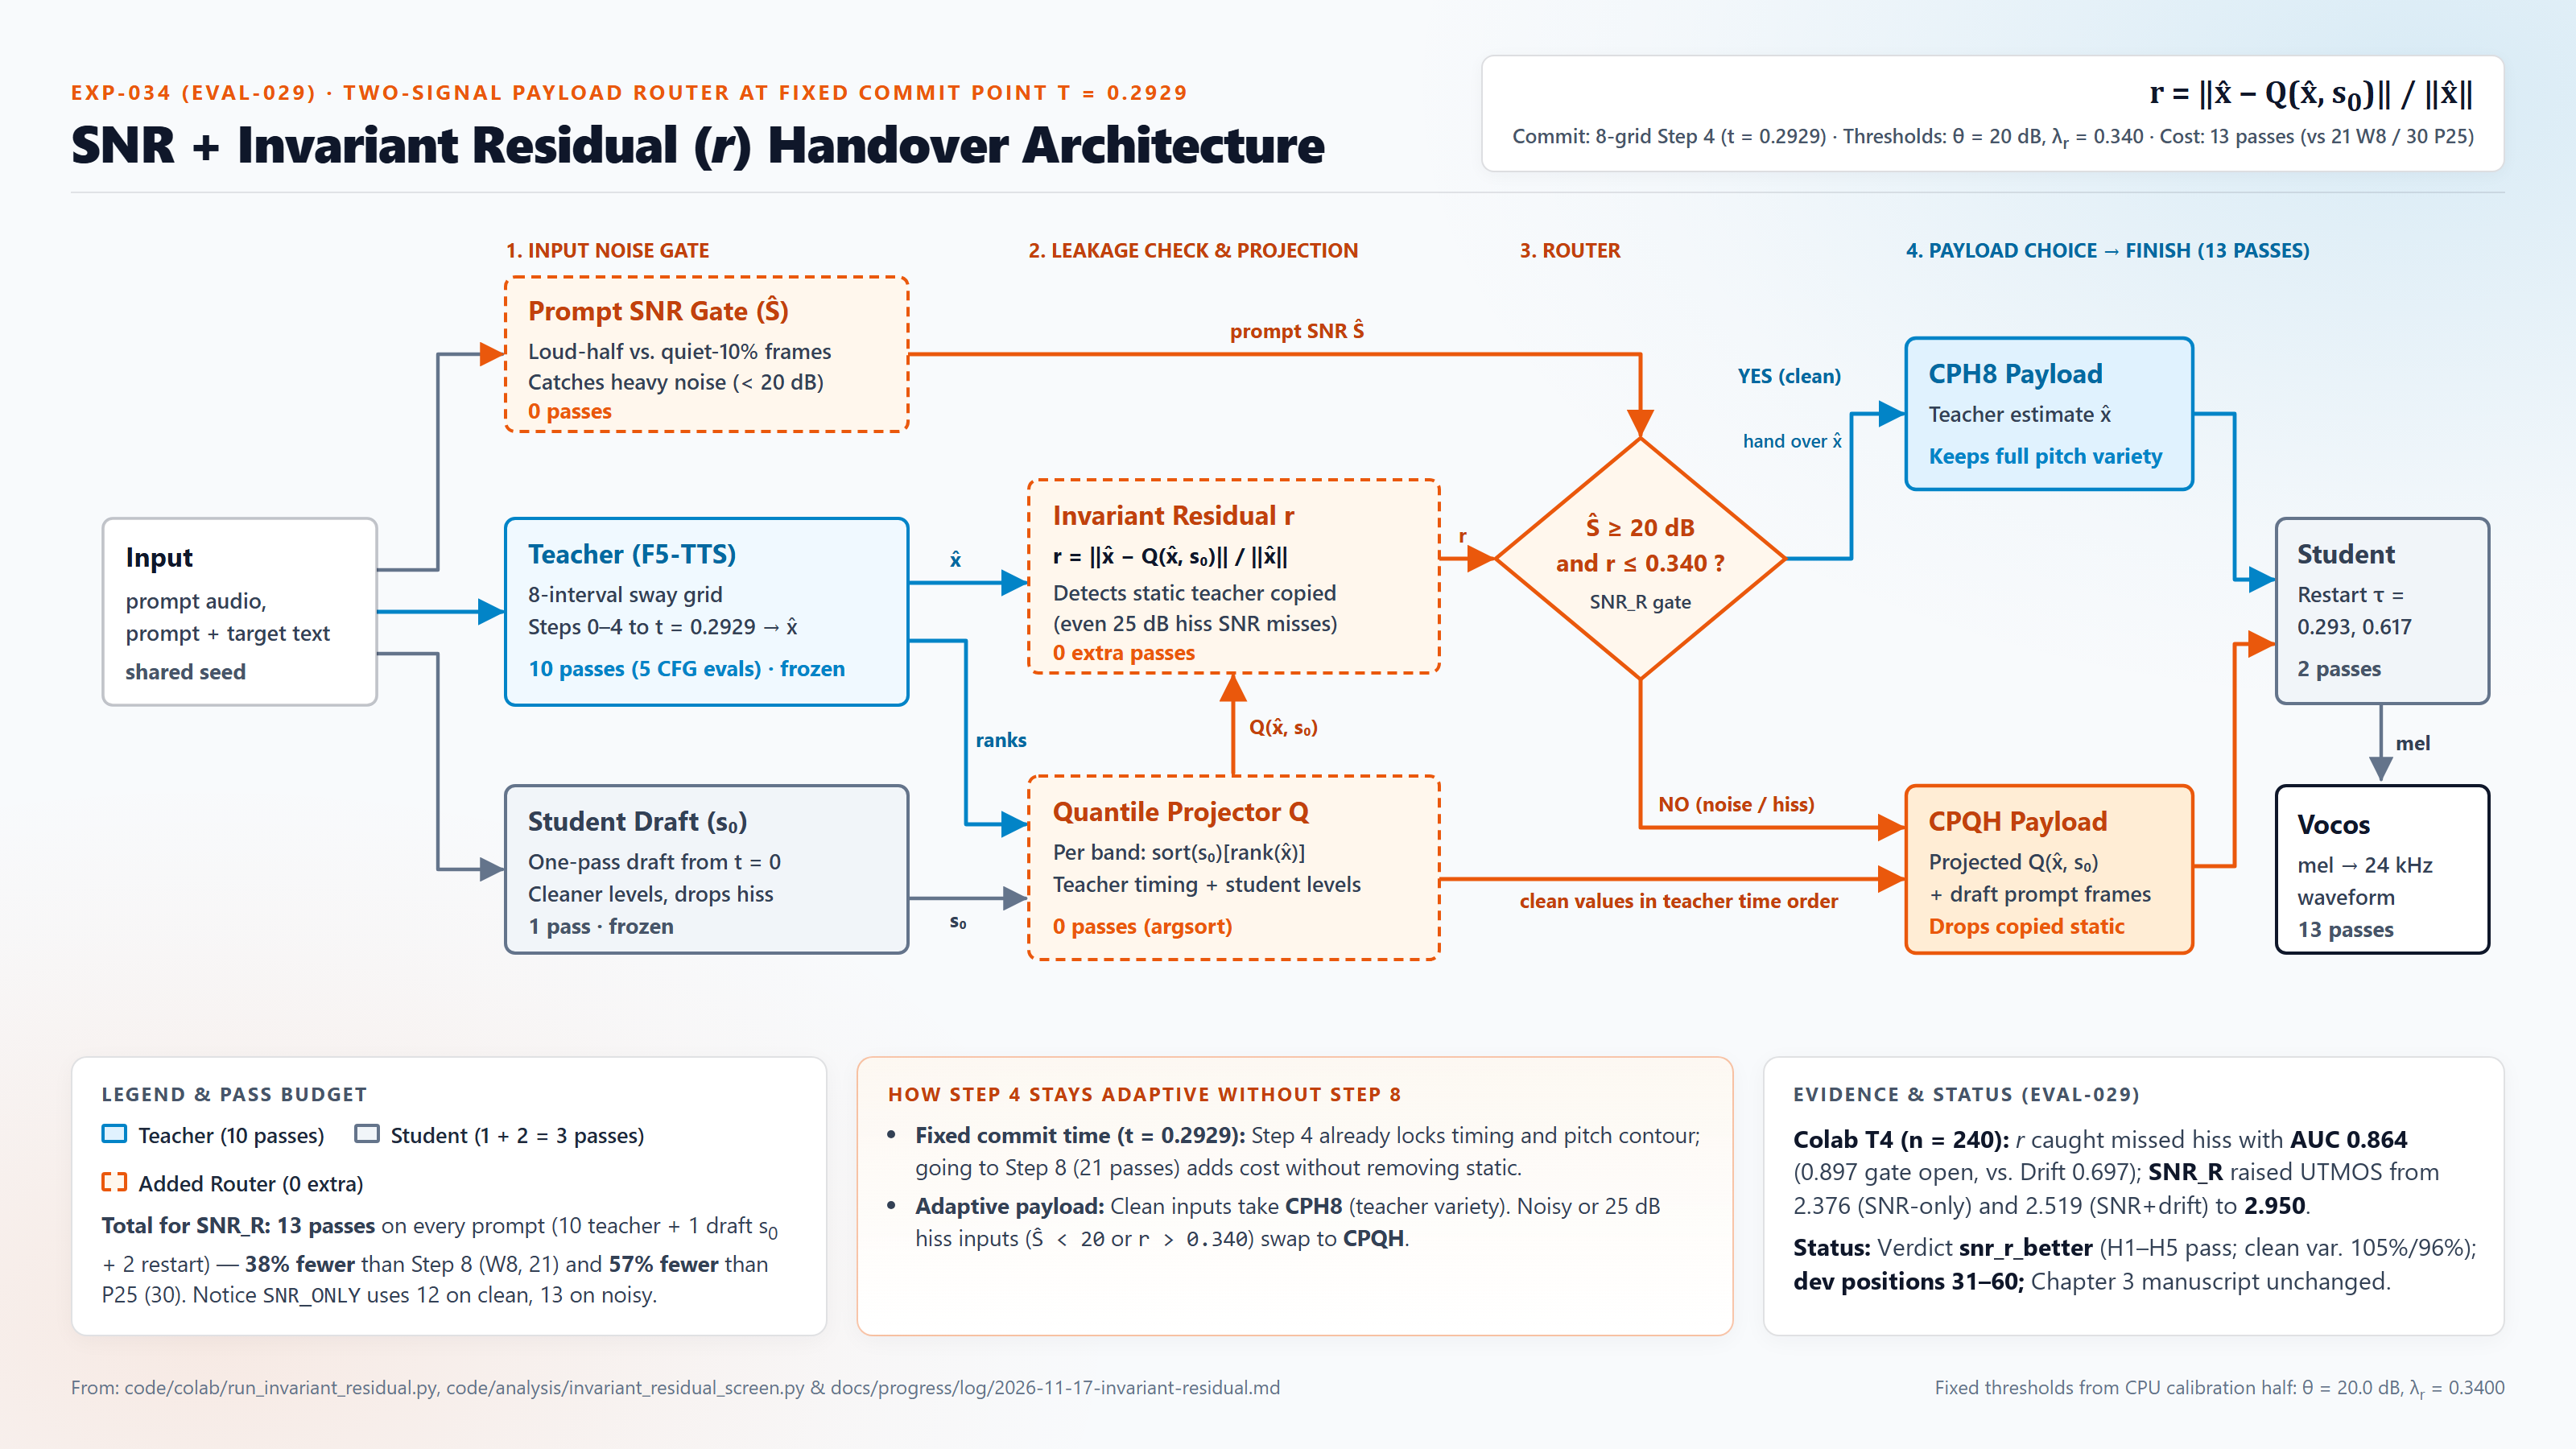
\includegraphics[width=\linewidth]{figures/exp034_architecture.png}
\caption[Architecture of the risk-calibrated (LTT) SNR and invariant residual (\texttt{SNR\_R}) handover router]{Architecture of the \texttt{SNR\_R} handover router in \texttt{EXP-034}}
\label{fig:snr-r}
\par\vspace{2pt}{\footnotesize\raggedright\textit{Note.} Architecture of the two-signal SNR and invariant residual (\texttt{SNR\_R}) handover router evaluated in \texttt{EXP-034} (updated with offline Learn-Then-Test risk calibration $\lambda_r^*=0.342$ at $\alpha\le 15\%,\ \delta=0.10$ and completed \texttt{EXP-034}/\texttt{EXP-035} Colab Tesla T4 outcomes; bottom-right box). Rather than choosing among teacher stopping steps $k\in\{4..8\}$ at $j=1$ as in Figure~\ref{fig:method}, the pipeline stops the 8-interval teacher at $t_4=0.2929$ (10 passes), generates the 1-pass student draft $s_0$, computes $r$ from the per-band quantile projection $Q(\hat x_1,s_0)$, and routes the handover payload between \texttt{CPH8} and \texttt{CPQH} before running the remaining two student passes at $j=2$ (13 passes total).\par}
\end{figure}
